%%%%%%%%%%%%%%%%%%%%%%%%%%%%%%%
%This is the article LaTeX template for RSC journals
%Copyright The Royal Society of Chemistry 2010
%%%%%%%%%%%%%%%%%%%%%%%%%%%%%%%


\documentclass[8.5pt,twoside,twocolumn]{article}
\oddsidemargin -1.2cm
\evensidemargin -1.2cm
\textwidth 18cm
\headheight 1.0in
\topmargin -3.5cm
\textheight 22cm
\usepackage[super,sort&compress,comma]{natbib} 
\usepackage{graphicx}
\usepackage{color}
\usepackage{mhchem}
\usepackage{times,mathptmx}
\usepackage{sectsty}
\usepackage{balance} 

\usepackage{graphicx} %eps figures can be used instead
\usepackage{lastpage}
\usepackage[format=plain,justification=raggedright,singlelinecheck=false,font=small,labelfont=bf,labelsep=space]{caption} 
\usepackage{fancyhdr}
\pagestyle{fancy}

\begin{document}

\thispagestyle{plain}
\fancypagestyle{plain}{
\fancyhead[L]{\textit{\small{\textbf{Redes Neuronales}}}}
\fancyhead[C]{\textbf{Trabajo Pr\'actico I }}
\fancyhead[R]{\textbf{Jennifer Maldonado}}\vspace{0.5cm}}
\renewcommand{\thefootnote}{\fnsymbol{footnote}}
\renewcommand\footnoterule{\vspace*{1pt}% 
\hrule width 3.4in height 0.2pt \vspace*{2pt}} 
\setcounter{secnumdepth}{5}



\makeatletter 
\def\subsubsection{\@startsection{subsubsection}{3}{10pt}{-1.25ex plus -1ex minus -.1ex}{0ex plus 0ex}{\normalsize\bf}} 
\def\paragraph{\@startsection{paragraph}{4}{10pt}{-1.25ex plus -1ex minus -.1ex}{0ex plus 0ex}{\normalsize\textit}} 
\renewcommand\@biblabel[1]{#1}            
\renewcommand\@makefntext[1]% 
{\noindent\makebox[0pt][r]{\@thefnmark\,}#1}
\makeatother 
\renewcommand{\figurename}{\small{Fig.}~}
\sectionfont{\large}
\subsectionfont{\normalsize} 

\fancyfoot{}
\fancyfoot[RO]{\footnotesize{\sffamily{1--\pageref{LastPage} ~\textbar  \hspace{2pt}\thepage}}}
\fancyfoot[LE]{\footnotesize{\sffamily{\thepage~\textbar\hspace{2.45cm} 1--\pageref{LastPage}}}}
\fancyhead{}
\renewcommand{\headrulewidth}{1pt} 
\renewcommand{\footrulewidth}{1pt}
\setlength{\arrayrulewidth}{1pt}
\setlength{\columnsep}{6.5mm}
\setlength\bibsep{1pt}

\twocolumn[
  \begin{@twocolumnfalse}
  \vspace{0.2cm}
  \noindent \normalsize{
        La hoja de c\'alculo denominada "clima\_numerico" contiene los mismos patrones
representados por sus valores numéricos originales (en el caso de los atributos
humedad y temperatura) o por valores enteros asociados a la categor\'ia
correspondiente (0=falso y 1= verdadero; 0=lluvioso, 0.5=nublado; 1=soleado).
Utilice los patrones de la hoja "clima\_numerico" para entrenar un perceptr\'on que
permita predecir, a partir de una condición clim\'atica dada, si se jugará al golf o no
  }
  \vspace{0.5cm}
  \end{@twocolumnfalse}
  ]


%\section{Introducci\'on}
\begin{itemize}
    \item Analice si se producen variantes con respecto a los par\'ametros del algoritmo de entrenamiento. 
        \\
        \\
        Se realiz\'o la ejecucion de 50 iteraciones por cada alfa, modificando la cantidad m\'axima de iteraciones
        de forma incremental, el ejercicio por tener pocos n\'umero de filas (patrones) convergi\'o a la soluci\'on
 sin llegar al m\'aximo n\'umero de iteraciones s\'olo para los alfa -0.5, 0.3, 0.4, 0.5. Es importante mencionar que 
los datos no se encontraban normalizados.
        
        \begin{table}[h]
        \small
        \caption{ Alfas, Promedio de Iteraciones, Cantidad de Aciertos (promedios) }
        \label{tbl:example}
        \begin{tabular*}{0.5\textwidth}{@{\extracolsep{\fill}}llll}
        \hline
        Aciertos (Promedio) & alfa & Ite $<$ Max\_It & Ite (Promedio)\\
        \hline
        2 & 0.5 & $50/50$ & 22.06 \\
        2 & 0.4& $50/50$ & 19.04  \\
        2 & 0.3 & $50/50$ & 24.2 \\
        2 & -0.5 & $1/50$ & 1 \\
        2 & 0.2 & $50/50$ & 25.5 \\
        2 & 0.1 & $50/50$ & 23.64 \\
        1.54 & -0.1 & $0/50$ & 2550 \\
        1.6 & -0.2 & $0/50$ & 2550 \\
        1.46 & -0.3 & $0/50$ & 2550 \\
        1.42 & -0.4 & $0/50$ & 2550 \\
        \hline
        \end{tabular*}
        \end{table}
        En todas las variaciones de alfa, se reduce el n\'umero de iteraciones siendo el alfa 0.4 el porcentaje de 
        aprendizaje que puede llegar a reducir el  n\'umero de iteraciones.

    \item Analice si es necesario escalar los datos de entrada. 
    \item ¿Es posible clasificar todos los patrones correctamente ingresando todos los de una clase primero y luego todos los de otra clase?
    \item A partir de los pesos del perceptron entrenado, indique cual es la funci\'on discriminante obtenida.
    \item seleccione dos patrones y calcule manualmente, para cada uno de ellos la respuesta del perceptron entrenado.
\end{itemize}

El Modelado de T\'opicos es una t\'ecnica para tratar documentos que no tienen alguna categorizaci\'on, esta t\'ecnica asume que cada documento es una mezcla aleatoria de categor\'ias o t\'opicos, donde cada categor\'ia es definida por la preferencia de algunas palabras sobre otras.
\\
\\
Un t\'opico en el contexto de modelado de t\'opicos es una distribuci\'on
de probabilidades de palabras para un conjunto, e indica la probabilidad
que una palabra aparezca en un documento  sobre un t\'opico en particular. Para obtener esto el modelado de t\'opicos asume que las palabras que comprende el texto fueron generadas aleatoriamente y no poseen relaci\'on alguna. Su objetivo es Inferir una convincente respuesta bajo la asunci\'on anterior.  
\\
\\
Los proyectos de Modelados de t\'opicos se dividen en:
\begin{itemize}
\item \emph{Proyectos de enfoque sincr\'onico}. 
          en el cual el valor de la unidad de an\'alisis no 
          posee l\'imite de tiempo, o mejor dicho no se 
          identifica con una brecha de tiempo.

\item \emph{Proyectos de enfoque diacr\'onico}. 
          La unidad de analisis de tiempo se genera 
          en un fecha o rango de fecha definido.
\end{itemize}
El Modelado de T\'opicos puede ser usado para clasificar documentos similares 
adem\'as permite mejorar la indexaci\'on de texto, pudiendose combinar con m\'etodos de 
recuperaci\'on de informaci\'on otra de sus aplicaciones consiste en identificar la evoluci\'on de ciertos t\'opicos sobre
un periodo de tiempo adem\'as de encontrar relaciones entre los diferentes t\'opicos.
Tambi\'en predecir citaciones en base a la presencia de t\'opicos similares en un texto.
\\ 
\\
Para evaluar que modelo de t\'opicos se ajusta mejor a los datos, muchos papers mencionan que es necesario 
ejecutar en N iteraciones dependiendo del objetivo del modelo si es algo muy general o muy espec\'ifico depende
de los par\'ametros que reciba el algoritmo. Otra medida  es la perplejidad por palabra que consiste
en la cantidad de bits utilizados para modelar un texto, en cuanto la perplejidad es menor se podr\'ia decir que
el modelo es m\'as espec\'ifico y se ajusta mejor al texto, por lo que se considera mejor 
tener un modelo con menor perplejidad.

\section{Preparaci\'on e Instalaci\'on}

%Footnotes
\footnotetext{\dag~ Script para formatear Git Hub: [http://bit.ly/15VZJBC].}

En cuanto a nutch y solr s\'olo requieren ser descargados y modificar los archivos de configuraci\'on  a medida de lo que se requiera, en nuestro caso necesitabamos que indexara p\'aginas que pertenecieran al mismo dominio. Adem\'as Requiere tener java instalado en la m\'aquina.
\\
El proceso de Descarga de los diarios se realiz\'o durante 2 semanas, sin embargo realizaremos modelado de t\'opicos sin tomar en cuenta la secuencia en que fueron publicados los art\'iculos. Luego del formato CSV obtenido a trav\'es del servidor Solr fue llevado al formato:
\\
Directorio/file1.txt \\
Directorio/file2.txt \\
\\
En el cual se importa la carpeta que contiene los archivos que servir\'an como
 entrenamiento para el modelado de t\'opicos. Luego se tom\'o un 10\% como muestra 
para realizar la evaluaci\'on e inferencia de nuevos t\'opicos. Los archivos usados 
para entrenamiento se encuentran en la carpeta \emph{train}, y los usados para evaluar el
modelo en la carpeta \emph{test} en el repositorio listado en las referencias.
\\
\\
En este trabajo utilizamos Mallet y la implementaci\'on que contiene del Algorithm LDA (latent Dirichlet allocation) para realizar el Modelado de t\'opicos, mediante el ajuste de las frecuencias de palabras  a la probabilidad a priori, y Gibbs Sampling para simular el c\'alculo de la probabilidad a posteriori, sin embargo se puede utilizar otro tipo de distribuci\'on en ambas etapas, editando par\'ametros de software Mallet. 
\\
\\
se realiz\'o el Modelado de t\'opicos en muchas iteraciones
 con diferentes par\'ametros para visualizar qur\'e combinaci\'on de 
par\'ametros ser\'ia la m\'as \'optima. Durante 4 iteraci\'ones se  a\~nadi\'o m\'as palabras al listado de stopwords, cabe destacar que Mallet no trae en su instalaci\'on por defecto con un listado de stopwords en espa\~nol. Sin embargo se pueden añadir una lista de stopwords en funci\'on del corpus.
\\
\\
Cada iteraci\'on consta de los siguientes procesos:
\begin{itemize}
\item \emph{Importar Archivos},
            Este proceso convierte los archivos 
            en formato directorio/file1.txt  al formato Mallet, para el 
            entrenamiento y evaluaci\'on del Modelo. 
\item \emph{Entrenamiento},
            Este proceso a trav\'es de los par\'ametros 
            configurados en Mallet realiza el entrenamiento 
            con el formato que arroj\'o el paso anterior. (entrenamiento\_unigram.sh)
\item \emph{Inferencia de nuevos datos},
            Teniendo el archivo con formato Mallet de los datos de test, 
            y el archivo del modelo de entrenamiento, obtenido en el paso anterior, 
            se realiza la asignaci\'on de t\'opicos a los documentos de \emph{test} (ver inferencer.sh)
            
\item \emph{Evaluacion de la inferencia},
            Mallet permite evaluar los modelos generados, a trav\'es del comando 
            evaluate-topics, esto toma como par\'ametro de entrada el archivo obtenido en 
            el anterior paso. Y permite visualizar que tan espec\'ifico o general es un modelo
            a trav\'es de la m\'etrica de perplejidad. (ver evaluate.sh)
\end{itemize}

Luego de haber cumplido el anterior proceso, graficamos la perplejidad y
 elegimos dos modelos, k=8 (k = n\'umero de t\'opicos) porque tiene  el mayor peso en uno de sus 
t\'opicos con respecto a todas las iteraciones y conserva la generalidad del modelo para asociar diarios.
 Y k=4 e i=10 ya que de acuerdo a la siguiente
 gr\'afica tiene el menor valor de la perplejidad en este n\'umero de t\'opico que es  m\'as general.

\begin{figure}[h]
  \centering
  %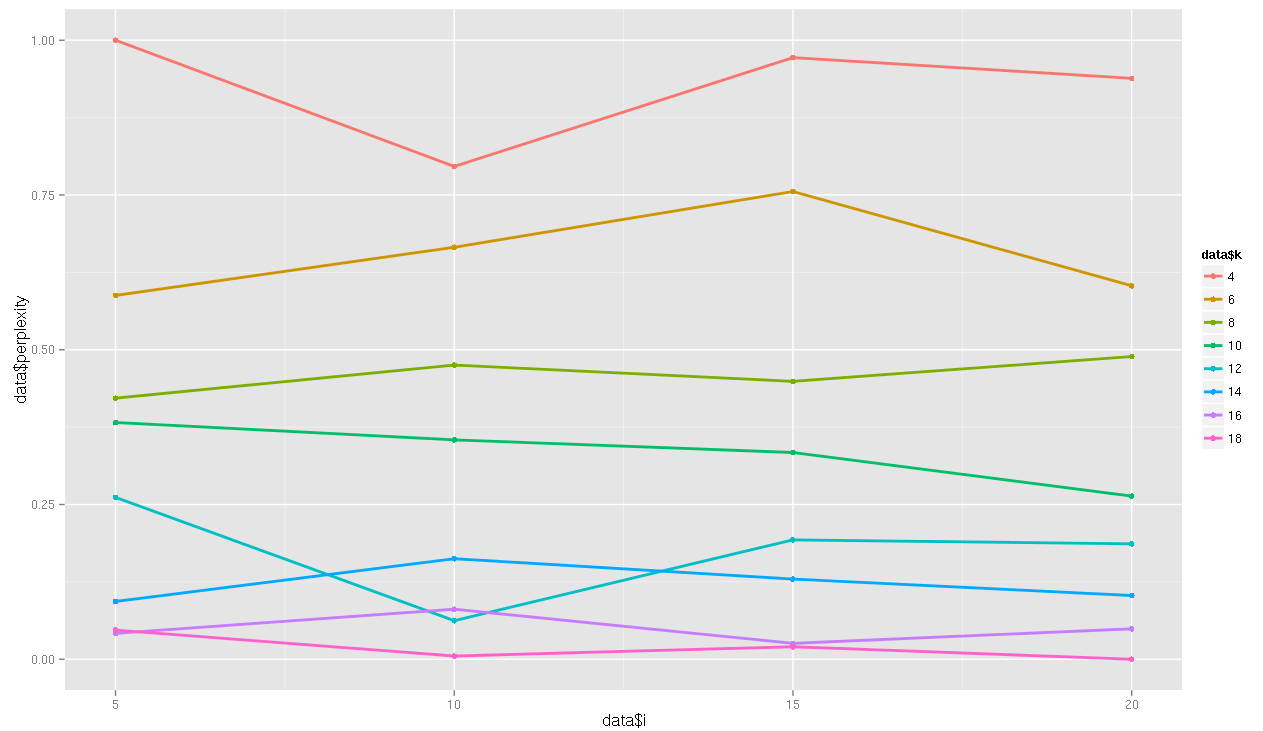
\includegraphics[scale=0.2]{perplexity.png}
  \caption{Perplejidad para cada iteraci\'on con la variaci\'on de k e i (par\'ametro que optimiza el modelado de t\'opico) } 
  \label{fgr:perplexity}
\end{figure}

Adem\'as se puede observar que a medida que incrementamos los tags se decrementa la perplejidad, 
por lo que es una medida que te permite definir si ser\'a mejor clasificador el modelo.
Para modelos m\'as generales la perplejidad  ser\'a mayor.

\subsection{ Visualizando m\'as de 10000 art\'iculos}
Los archivos generados por Mallet luego de su entrenamiento son:
\begin{itemize}
\item \emph{noticias\_keys.txt}, tiene un listado de los t\'opicos , y a cada t\'opico le asigna un peso, de acuerdo a su relevancia. hicimos un gr\'afico de c\'irculos donde el di\'ametro del c\'irculo corresponde al peso del t\'opico.  
\item \emph{noticias\_composition.txt}, hicimos un treemap limitando el n\'umero de documentos a incluir por t\'opico, ya que el n\'umero de documentos es muy alto.
\item word-topic-count-files.txt, con este archivo realizamos el grafo de la distribuci\'on de palabras a trav\'es de los t\'opicos.
      Este grafo se realiz\'o tomando un l\'imite de probabilidades ya que son muchos documentos.
\item noticias\_inferencer.txt, muestra el t\'opico asignado a el nuevo documento.
\item \emph{noticias\_evaluator.txt}, Permite obtener m\'etricas para evaluar el Modelo, entre ellas la perplejidad.
\end{itemize}

\subsection{ Gr\'aficos de burbujas para T\'opicos para k=8  }
\begin{figure}[h]
  \centering
  %\includegraphics[scale=0.2]{burble_k8_5_mallet_keys.png}
  \caption{T\'opicos y sus Pesos.}  
  \label{fgr:perplexity}
\end{figure}

El t\'opico m\'as relevante, de acuerdo a su frecuencia de aparici\'on es el tema del cepo cambiario.  
Puede deberse a incluir mayor cantidad de diarios de Argentina que del resto del mundo.  
Otro t\'opico que destaca, menciona la crisis y deficit en europa.  
Al hablar de petr\'oleo, reformas, chav\'ez y crisis se asocia a Venezuela. 
Y el t\'opico que muestra temas como t\'opicos guerra, snowden, amenaza, usd, gas se asocia a Rusia.

\subsection{ Gr\'aficos de burbujas para T\'opicos para k=4  }
\begin{figure}[h]
  \centering
  %\includegraphics[scale=0.2]{burble_k4_10_mallet_keys.png}
  \caption{T\'opicos y sus Pesos.}  
  \label{fgr:burble}
\end{figure}

T\'opicos de la figura 3:
Dolares, Blue, fernandez, inflaci\'on, crisis, seguridad es el t\'opico con mayor peso y asocia a todos los diarios de argentina.
\\
Crisis en europa, deuda y deficit, representan a los diarios espa\~noles. 
\\
Venezuela, mundial, unidos, america latina, guerra, snowden, dolares, crisis, amenaza, acuerdos, china. Asocia a los diarios de actualidadRT.com
y avn.info.ve, puede deberse a que ambos pa\'ises ofrecieron asilo a snowden.

\subsection{ Grafo con la distribuci\'on de palabras por t\'opicos para k=4  }

Se puede observar en la figura 5 que el t\'opico 3 contiene un n\'umero mayor de palabras con respecto a los otros t\'opicos.
Siento este t\'opico m\'as general: crisis crecimiento reforma america centro venezuela desarrollo latina 
ministro plan mayor deuda mundial comercio inversiones economico problemas rol unidos.

\begin{figure}[h]
  \centering
  %\includegraphics[scale=0.2]{topics_words_4_10_txt.png}
  \caption{Distribuci\'on de Palabras por t\'opico, para k=4.}  
  \label{fgr:perplexity}
\end{figure}

\subsection{ Treemap para k=8  }

\begin{figure}[h]
  \centering
  %\includegraphics[scale=0.2]{tremap_k8_5_P0_998_unigram.png}
  \caption{Treemap para k=8, el color representa un t\'opico, y como agrupa los diferentes diarios.}  
  \label{fgr:treemap}
\end{figure}

 avn.info.ve, telegrafo.com.ec, eleconomista.com.mx, tienen los t\'opicos: centro venezuela
 desarrollo chavez interes america mundial muertos comercio latina
 politicas acuerdo eeuu redaccion revolucion crisis region snowden unidos. 	
\\

 ultimahora.com, cincodias.com, los asocia con los t\'opicos: europa credito asuncion
 fiscal inversiones rosalia subidas egipto depositos impuestos diaz palacio gibraltar. 
En este t\'opico debe asociar a diarios de paraguay s\'olo que no son listado por no 
tener una probabilidad de pertenencia por encima de 0.998
\\
 
 elpais.com, nuevatribuna.com menciona: euros alta crisis america europa fiscal 
deuda reforma  debate barcelona ministro partido 
medidas deficit paga bruselas francia bankia.
\\
el resto de los diarios de Argentina los asocia con el t\'opico 2, dolares precios 
inflacion cristina blue pesos menos crecimiento productos mayor maria 
crisis acuerdo oficial demanda bolsa credito argentinos deuda.


\section{Conclusiones.}
El potencial del modelado de t\'opicos no se observa en cada 
documento individualmente, sino m\'as bien en un enfoque global analizando 
grandes cantidades de documentos para visualizar patrones entre ellos. 
\\
\\
El Parametro DirichLet permite darle un peso al t\'opico, haciendo 
que sobresalgo por encima de otros t\'opicos, y la variacion de este 
parametros permite un mejor ajuste del modelo.
\\
\\
El intervalo permite que el software realice un calculo optimizado de los parametros alfa y beta cada N iteraciones.
\\
\\
Conforme se a\~naden m\'as t\'opicos el modelo se vuelve m\'as espec\'ifico, y tiende a colocar todos los documentos que pertenecen a un diario en un mismo t\'opico, para k=10, ocurri\'o esto, de 10 t\'opicos 8 ten\'ia una probabilidad alta por encima de 0.998 y 7 t\'opicos estaban asociados a un solo diario.
\\
\\
No existe un modelo mejor que otro, depende del objetivo. Si se desea realizar
\\
\\
 una clasificador de texto en base al modelado de t\'opicos, 
podr\'iamos usar k=cantidad de clases y modificar los parametros que permitan 
reducir la perplejidad al m\'aximo, de forma que cada t\'opico pueda representar una clase.
\\
\\
luego de cada ejecuci\'on, siempre arrojar\'a resultados diferentes ya que Mallet utiliza Gibbs sampling por defecto, para calcular la probabilidad a posteriori. Por ende la comparaci\'on entre modelos no es muy pr\'actica.
\\
\\
La cantidad de t\'opicos recomendada no existe por ende se debe realizar una gran cantidad de iteraciones para observar cual se ajusta mejor a la data. Usualmente mientras m\'as general menor cantidad de t\'opicos mientras m\'as espec\'ifico cada t\'opico tendr\'a menor cantidad de diarios.

\section{Referencias.}

\begin{itemize}
\item{Lista de Desarrollo Mallet} http://comments.gmane.org/gmane.comp.ai.mallet.devel/1294
\item{Modelado de Topicos, Universidad de Princeton} http://www.cs.princeton.edu/~blei/topicmodeling.html
\item{Topic Modelling with MALLET} http://hublog.hubmed.org/archives/001870.html
\item{Comprehending the Digital Humanities} https://dhs.stanford.edu/comprehending-the-digital-humanities/
\item{Gephi + MALLET + EMDA} http://www.robincamille.com/
\item{Identifying the pathways for meaning circulation using text network analysis} http://noduslabs.com/research/pathways-meaning-circulation-text-network-analysis/ 
\item{Redes de T\'opicos} https://dhs.stanford.edu/visualization/topic-networks/
\item{Review Mallet} http://journalofdigitalhumanities.org/2-1/review-mallet-by-ian-milligan-and-shawn-graham/
\item{Visualizing Topic Models with Force-Directed Graphs} http://tedunderwood.com/2012/12/02/visualizing-topic-models-with-force-directed-graphs/
\item{Mallet Paper} http://courses.washington.edu/ling572/winter2013/slides/class2\_570\_mallet.pdf
\item{SIGKDD 2011 Conference}http://www.bytemining.com/2011/08/sigkdd-2011-conference-day-1-graph-mining-and-david-bleitopic-models/
\item{C\'odigo Empleado en este trabajo Pr\'actico} http://github.com/j3nnn1/topic\_model
\item{Slides en HTML sobre Modelado de T\'opicos} http://j3nnn1.github.io/homework/tp\_textII/slides/topic\_modeling.html
\item{Perplejidad } http://es.wikipedia.org/wiki/Perplejidad

\end{itemize}

\footnotesize{
%\bibliography{rsc} %your .bib file
%\bibliographystyle{rsc} %the RSC's .bst file
}

\end{document}
